%% Version 2022-07-08
%% LaTeX-Vorlage für Abschlussarbeiten
%% Erstellt von Nils Potthoff, ab 2020 erneuert und ausgebaut von Simon Lohmann
%% Lehrstuhl Automatisierungstechnik/Informatik Bergische Universität Wuppertal
%%%%%%%%%%%%%%%%%%%%%%%%%%%%%%%%%%%%%%%%%%%%%%%%%%%%%%%%%%%%%%%%%%%%%%%%%%%%%%%%

\chapter{Datengrundlage}
	
	% 1) Intro: Daten wichtig für Wärmewende und Wärmepläne
	% 2) Recap: Welche Daten nötig, Verweis vorher
	% 3) Dieses Kapitel: Sichtung und Bewertung
	% 4) Vorschau: Überblick: Welche Daten -> Welche Datenquelle, Verweis Subkapitel
	% 5) Vorschau: Beschreibung Datenquellen [Auflösung, Genauigkeit, Abdeckung, Aktualität], Verweis Subkapitel
	
	% Intro: Warum Datengrundlage
	Für die Wärmewende ist eine detaillierte Datengrundlage essentiell, da sich nur mit umfangreicher Datenbasis optimal auf die jeweilige Region zugeschnittene Wärmewendestrategien entwickeln und umsetzen lassen. Hierfür bieten Wärmeplanungen einen holistischen Ansatz zur Strategie-Entwicklung, um der zunehmende Komplexität unserer Energie- und Wärmeinfrastruktur durch stetig wachsende Inter-Konnektivität der einzelnen Sektoren gerecht zu werden.
	
	% Inhalt dieses des Kapitels - Zweiteilig
	Im Zuge dieser Arbeit wird zur Erstellung einer geeigneten Datengrundlage eine Sichtung öffentlich verfügbarer Daten durchgeführt, welche daraufhin auf ihre Eignung hin bewertet und selektiert werden. Der Sichtungs-, Bewertungs- und Auswahlprozess für Daten wird im ersten Teil dieses Kapitels in \autoref{sec:Daten:Aquise} beschrieben. Eine detailliertere Beschreibung des Inhalts, des Formats, möglicher Anwendungsfelder und der Bewertung auf Eignung der ausgewählten Datensätze erfolgt im zweite Teil dieses Kapitels in \autoref{sec:Daten:Datensatz}. 
	
	\section{Sichtungsprozess und Daten-Aquise}
	\label{sec:Daten:Aquise}
		% 1) Was für Daten gebraucht?
		% 2) Vorraussetzungen und Bewertungskriterien allgemein
		% 3) Sichtungsprozess (wo suchen?)
		% 4) Überblick ausgewählter Datensätze
		Für die Auswahl von Datensätzen für eine geeignete Datengrundlage wurde zunächst eine Liste erstellt, welche Daten erforderlich für Wärmeplanungen sind. Die Zusammenstellung ist in \autoref{sec:Daten:Aquise:Erforderliche_Daten} beschrieben und orientiert sich an den Prozessschritten von Wärmeplanungen. 
		
		Als nächsten Schritt wurden allgemeine Voraussetzungen und Bewertungskriterien definiert, um begutachtete Datensätze auf ihre Eignung für Wärmeplanungen zu bewerten. Die definierten Voraussetzungen und Bewertungskriterien finden sich in \autoref{sec:Daten:Aquise:Bewertungskriterien}.
		
		Daraufhin werden in \autoref{sec:Daten:Aquise:Sichtung} der eigentliche Sichtungsprozess beschrieben und mögliche Datenquellen aufgezählt, die im Laufe der Arbeit begutachtet wurden. 
		
		Zum Schluss wird das vorläufige Ergebnis der Sichtung in Kapitel \autoref{sec:Daten:Aquise:Überblick} anhand einer Tabelle mit Gegenüberstellung von Anwendungszweck und jeweils nutzbarem Datensatz präsentiert. 
		
		\subsection{Erforderlicher Daten}
		\label{sec:Daten:Aquise:Erforderliche_Daten}
			% Aufbau: Wofür welche Daten?
			Um eine geeignete Datengrundlage für Wärmeplanungen zusammen zu stellen wurde zunächst eine Liste erforderlicher Daten zur Bestandsaufnahme, dem ersten Schritt einer Wärmeplanung, kreiert. Zur besseren Orientierung wurde eine grobe Unterteilung vorgenommen hinsichtlich Daten zur Gemeindestruktur und Daten zu Energie- bzw. eine daraus abgeleiteten Treibhausgas-Emissions-Bilanzen. \\
			
			\textbf{Bestandsaufnahme-Daten umfassen z.B. Daten zu:}
			\begin{itemize}
				\item Gemeindestruktur
				\subitem Kommunale Daten (Verwaltungsgrenzen, Population)
				\subitem Gebäudebestand (Art, Alter, Dämmstandard, Population, Größe, Heizsystem)
				\subitem Gebiets-Nutzungsart (Wohngebiet, Industrie, Gewerbe, etc.) (Flächennutzungspläne)
				\subitem Netze, bestehend und geplant (Wärme, Gas, Glasfaser)
				\subitem Schutzgebiete (z.B. Natur-, Landschafts-, Naturata2000-, FFH-, Vogel-, Wasser-Schutzgebiete)
				\item Energie- und THG-Emissions-Bilanz
				\subitem Erzeugungsdaten (nach Energieträger)
				\subitem Verbrauchsdaten (nach Energieträger / Sektor)
				\subitem THG-Emissionen (nach Energieträger / Sektor)
			\end{itemize}
			
			% Potentialanalyse: Welche Daten?
			Im Zweiten Schritt der Wärmeplanung werden zur Erstellung einer Potentialanalyse Daten zu potentiellen Wärmequellen einer Region gesammelt. Zur Strukturierung bietet sich die Aufteilung nach Energieträgern an. \\
			
			\textbf{Potentialanalyse-Daten umfassen z.B. Daten zu:}
			\begin{itemize}
				\item Potentiale zur Wärme-Erzeugung nach Energieträger
				\subitem Biomasse (nachwachsend, Klär-, Bio- oder Deponiegas)
				\subitem Geothermie (oberflächennah, (mittel-)tief, Grubenwasser)
				\subitem Solarthermie (Freiflächen, Dachflächen)
				\subitem Umwelt-Wärme (Oberflächenwasser, Luft)
				\subitem Abwärme (Industrie und GHD, Rechenzentren, Abwasser, Müllverbrennung, KWK-Anlagen, Power-to-X-Anlagen)
				\item Potentiale zur Strom-Erzeugung nach Energieträger
					\subitem Wind (onshore, offshore)
					\subitem PV (Freiflächen, Dachflächen)
					\subitem Wasser (Fließwasser-, (Pump-)Speicher-Kraftwerke)
			\end{itemize}	
			
			Von weiteren Daten zur Aufstellung von Zielszenarien und Wärmewendestrategien, den Schritten drei und vier für Wärmeplanungen, wurde in dieser Arbeit aus Zeitgründen und dem geplanten Umfang der Arbeit abgesehen. 
			
		\subsection{Vorraussetzungen und Bewertungskriterien}
		\label{sec:Daten:Aquise:Bewertungskriterien}
			% Intro: Bewertungskriterien Beschreibung zur Eingrenzung
			Die Kriterien zur Bewertung der Eignung gesichteter Daten sind nach eigener Definition deren öffentliche Zugänglichkeit, inhaltlich u.A. deren Relevanz, Genauigkeit, räumliche Auflösung, ihr räumlicher Abdeckungsgrad, ihre Aktualität und prozesstechnisch deren Kompatibilität, Größe, Prozessierbarkeit und Performance bei der Verarbeitung je nach Formatierung. Relevanz in diesem Kontext bedeutet, dass die untersuchten Daten in einem der vier Wärmeplanungs-Prozessschritte verwendet werden können, also in der Bestandsaufnahme, Potentialanalyse, Szenarien-Entwicklung oder Wärmewendestrategie hilfreich sind. 
			
			% Hinweis: Verfügbarkeit
			In Bezug auf die Verfügbarkeit ist anzumerken, dass im Zuge dieser Arbeit wie im Themenblatt spezifiert lediglich öffentlich zugängliche Daten ausgewertet wurden. Für konkrete Wärmeplanungen haben Kommunen gegebenenfalls Zugang zu weiteren Daten. Dazu können kommuneninterne Daten gehören oder je nach Landesgesetzgebung beispielsweise auch gebäudescharfe Verbrauchsdaten von Versorgungsunternehmen wie in Baden-Württemberg. 
			
			Bezüglich der Auflösung von Daten sind für lokale Wärmeplanungen stets höchst mögliche Auflösungen vorzuziehen. Daten können beispielsweise gebäude-/anlagenscharf vorliegen oder aggregiert z.B. für Gitterzellen oder andere Gebietsunterteilung wie verwaltungstechnische Einheiten à la Gemeinden, Kreise, etc.. 
				
			% Hinweise zu Abschätzung bei nicht verfügbaren Daten:
			Im Idealfall liegen erforderliche Daten direkt in geeigneter Form vor. Andernfalls sollten sich vorliegende Daten zumindest dafür eignen, um Abschätzungen zu treffen, z.B. indem Rückschlüsse auf erforderlicher Daten getroffen werden können. Im Folgenden sind exemplarisch ein paar Beispiele genannt für geeignete Daten zur Prognose von Verbräuchen und verschiedener Potentiale. Die mögliche Eignung von Daten muss hierfür in jedem Fall einzeln bewertet werden.
			
			Für Wärmeplanende ohne Zugriff auf direkt erhobene Verbrauchsdaten könnten sich beispielsweise Daten zum Gebäudebestand wie Gebäudegröße und -funktion für Verbrauchsabschätzungen eignen. Ähnliches gilt auch in Bezug auf die Abschätzung des Dämm- bzw. energetischen Modernisierungspotentials. Liegen keine Daten zu durchgeführten energetischen Modernisierungsmaßnahmen vor, bietet sich z.B. die Analyse der Altersstruktur des Gebäudebestandes als Indikator an. Für die Abschätzung des erschließbaren Potentials neuer Wärmequellen müssen in der Regel ohnehin Annahmen getroffen werden falls diese noch nicht in Studien vorgenommen wurden. Indikatoren für das Geothermiepotential können z.B. u.a. geologische Auswertungen wie die Wärmeleitfähigkeit, die Untergrundtemperatur und hydrogeologische Sensibilität sein oder für Solarpotentiale z.B. u.a. die Globalstrahlungsintensität, die durschnittliche Sonnenscheindauer, die Topographie, die Gebäudegeometerien vorhandener Gebäude und die Geometrie des Baumbestandes (aufgrund von möglicher Verschattung) sein. 
			
			
			%versucht werden, diese möglichst genau zu prognostizieren.
			%Die zu verwendenen Daten müssen Hinweise auf den spezifischen Wärmeverbrauch je Quadratmeter Wohn-/Nutzfläche und Jahr und/oder je Meter Straßenzug und Jahr liefern. Im Idealfall auch gleich potentielle Wärmequellen mit anzeigen, sei es durch noch ungenutzte Abwärme oder nicht erschlossenen Photothermie- oder Geothermie-Potentialen.\\
			
			%... oder Sanierungspotential oder Erzeugungspotential, oder sowas z.B. ...\\
			
			%Dies kann entweder direkt durch bereits getroffene Abschätzungen erfolgen (Wärmeverbrauchs-studien) oder indirekt durch Auswertung von Daten zum Gebäudebestand (Alter, Dämmstandard, ...) und der Bewohnungsdichte erfolgen. Wobei hierfür Daten mit Geo-Bezug zum Erstellen detaillierter Karten hilfreich sind.\\
			
			%Eine Vorraussetzung zur Verwendung von Daten innerhalb dieser Arbeit ist der offene Zugang zu diesen. \\
			
			%Die Arbeit beschränkt sich des weiteren auf Daten für das Bundesland Nordrhein-Westfalen.\\
			

		\subsection{Sichtungsprozess und mögliche Datenquellen}
			\label{sec:Daten:Aquise:Sichtung}
			Für die Sichtung der Datenquellen wurden im Zuge dieser Arbeit Leitfäden und Informationsplattformen mehrerer Landesbehörden herangezogen (BW \cite{kea_bw_leitfaden_waermeplanung}, NRW \cite{web_energieatlas}, Niedersachsen \cite{web_leitfaden_waermeplanung_datenquellen_niedersachsen}), eigene Recherchen durchgeführt und beispielhaft genannte Quellen für Geodaten meines Betreuers betrachtet. 
			
			Zu den untersuchten Portalen zur Akquirierung geeigneter Daten für Wärmeplanungen mit Geobezug wurden u.A. die Webpräsenzen der folgenden Institutionen betrachtet:
			
			\begin{itemize}
				\item \textit{OpenGeodata.NRW} \cite{web_download_opengeodata_nrw}
				\item Zensus2011, Mikrozensus \cite{web_zensusatlas}
				\item Marktstamm-Register \cite{web_mastr}
			\end{itemize}
	
			% Anerkennung Vorarbeit von LANUV, KEA-BW und statistischen Ämtern, Bund und Länder
			Landesbehörden wie das LANUV und die KEA-BW haben bereits hervorragende Arbeit geleistet in der Aufbereitung von Daten für Wärmeplanung und Bereitstellung von Informationen zu deren Durchführung. Da in der Arbeit zwar bundesweit verfügbare Daten gesichtet wurden, aber der Fokus auf NRW gelegt werden sollte, wurden vielfach NRW spezifische Daten u.a. aus verschiedenen Studien des LANUV herangezogen.  
	
			% Eingrenzung der Arbeit und Verweis zu weiterführender Literatur
			Aufgrund des begrenzten Umfangs dieser Arbeit ist darauf hinzuweisen, dass keine umfassende Analyse zu sämtlichen verfügbaren Datenquellen durchgeführt werden kann. Für weitere Recherchen sei daher die Leitfäden der KEA-BW und der KEA-Niedersachsen verwiesen. Dort werden sowohl durch die Landesgesetzgebung für Gemeinden garantierte Datenquellen wie Verbrauchsdaten von Einwohner*innen bei Energieversorgungsunternehmen und Schornsteinfeger*innen (in BW) erwähnt, als auch öffentlich zugängliche Daten verschiedener Typen und Quellen aufgeführt. \cite{kea_bw_leitfaden_waermeplanung} \cite{web_leitfaden_waermeplanung_datenquellen_niedersachsen}
			
			% OpenGeodata.NRW
			Die umfangreichste in dieser Arbeit betrachtete und für Wärmeplanungen nützliche Datenquelle mit Geobezug für NRW bietet das Online-Portal \textit{OpenGeodata.NRW} des Landesbetrieb Information und Technik Nordrhein-Westfalen.\\
		
		\subsection{Überblick zu Datenquellen nach Anwendungsbereich}
		\label{sec:Daten:Aquise:Überblick}
			% Aufbau Überblick	
			Um einen Überblick über gesichtete Datenquellen mit möglichen Anwendungsbereichen zu geben, wurde im Laufe des Sichtungsprozess eine Übersichtstabelle erstellt. Da bis zum Ende dieser Arbeit noch keine abschließende Sichtung für Potential-Daten vorgenommen werden konnte, sind in \autoref{tab:Datengrundlage_Überblick} lediglich Datenquellen und mögliche Anwendungsbereiche für die Bestandsaufnahme von Wärmeplanungen gezeigt. Die Daten sind wie in \autoref{sec:Daten:Aquise:Erforderliche_Daten} beschrieben untergliedert. Ausgegraute Datensätze wurden nicht verwendet. 
			
			
			%Für die Bestandsaufnahme im Zuge von Wärmeplanungsprozessen ist in \autoref{tab:Datengrundlage_Überblick} ein Überblick zu möglichen Datenquellen gegeben. Die Tabelle bietet eine übersichtliche Zusammenfassung zu verfügbaren Datensätzen, unterteilt in die Bereiche Gemeindestruktur, Energie-Erzeugung, Energieverbrauch und THG-Emissions-Bilanz. 
						
			%für verschiedene Bereiche mit einer kurzen ergänzenden Beschreibung des Inhalts, Anmerkungen zum Format 
			
			\begin{table}[H]
				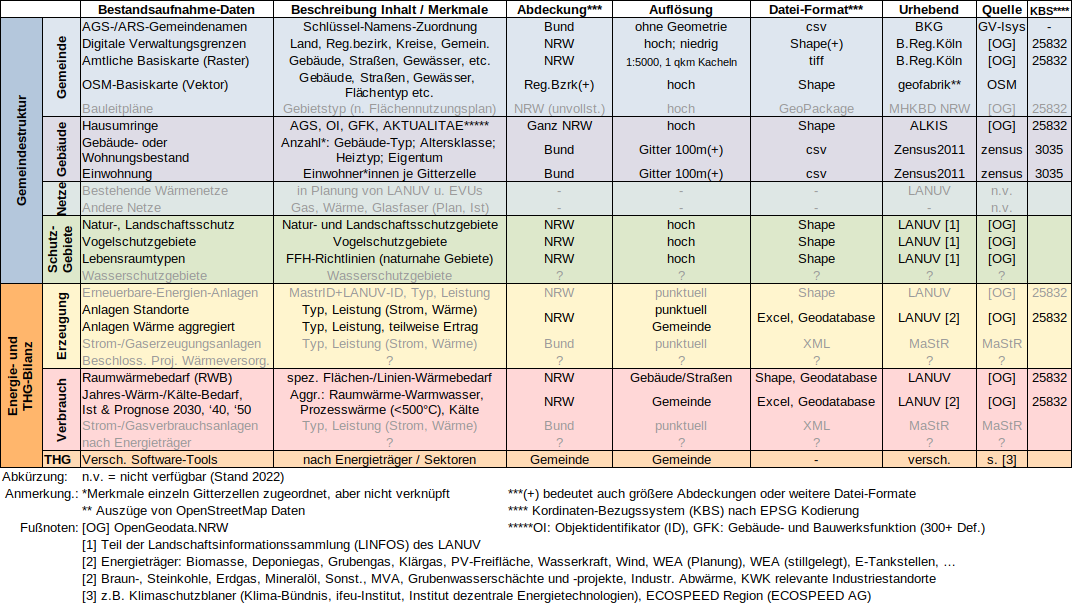
\includegraphics[width=1.00\textwidth]{Medien/tables/Datengrundlage_Ueberblick.png}
				% options neben width: page=1, angle=90
				\caption{Anwendungsfälle und Datenquellen im Überblick}
				\label{tab:Datengrundlage_Überblick}
			\end{table}
		
			%\begin{table}[H]
		%		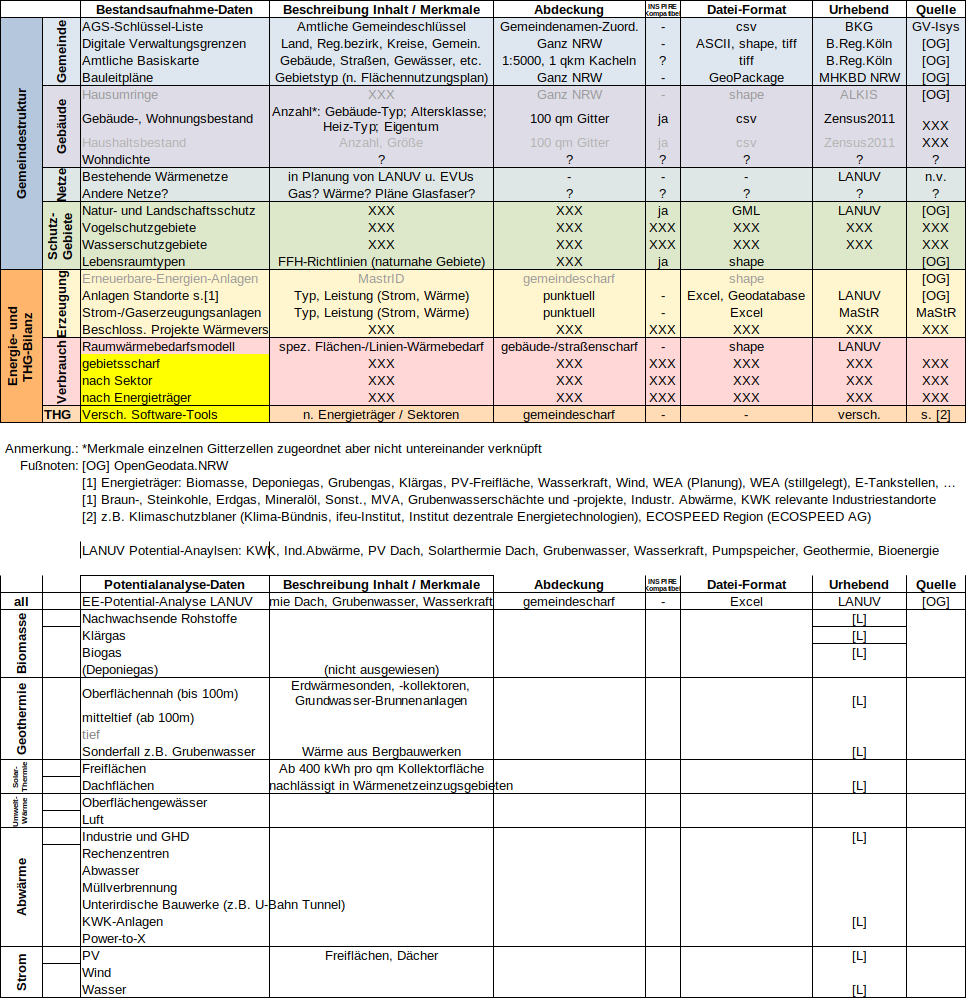
\includegraphics[width=1.00\textwidth]{Medien/tables/Datengrundlage_Ueberblick_big.png}
		%		\caption{Anwendungsfälle und Datenquellen im Überblick}
		%		\label{tab:Datengrundlage_Überblick_big}
		%	\end{table}
		
					
		%	\begin{figure}[H]
		%		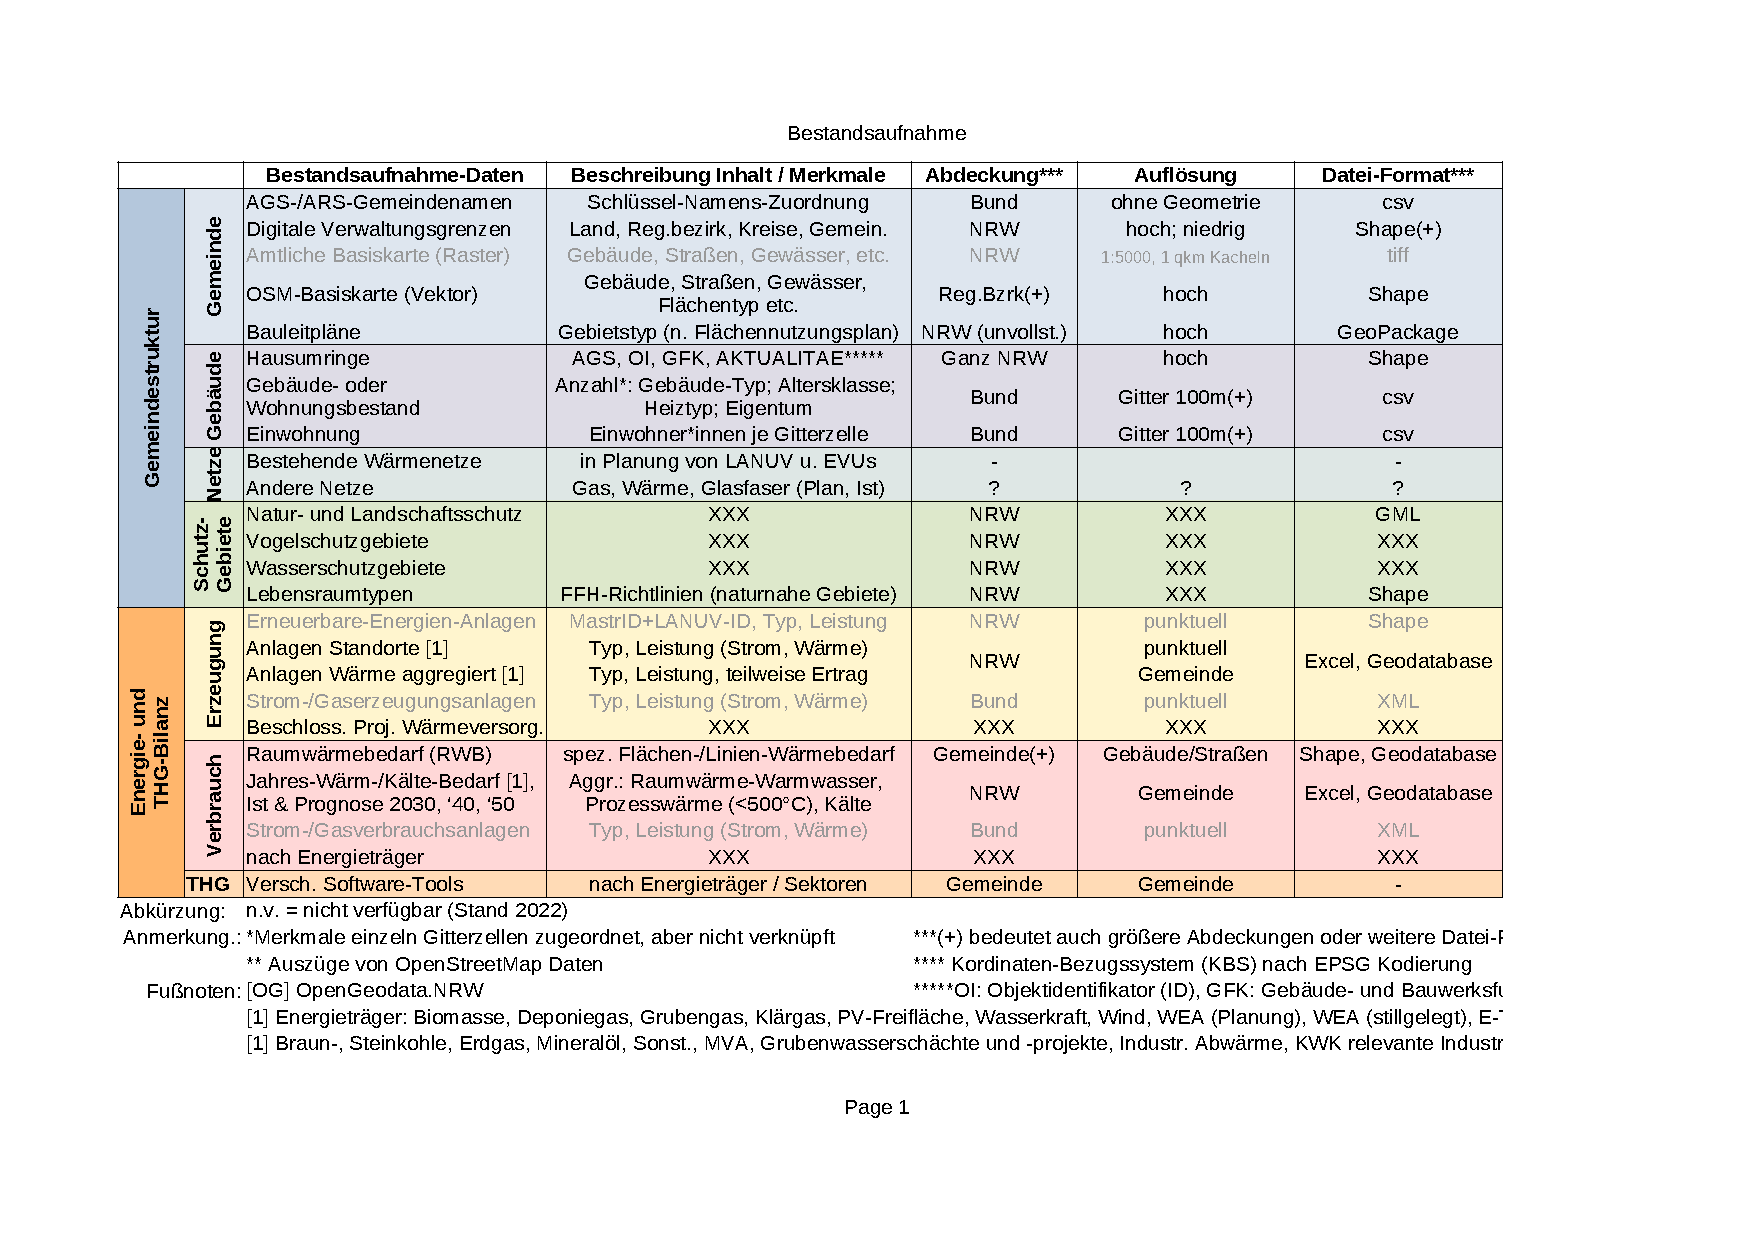
\includepdf[landscape=true, pages=1]{Medien/tables/Datengrundlage_Ueberblick.pdf}
		%		\caption{Anwendungsfälle und Datenquellen im Überblick}
		%		\label{tab:Datengrundlage_Überblick}
		%	\end{figure}
			
			
			%Aufgezählt werden Inhalt, Datei-Format, Koordinatenbezugssystem und gegebenenfalls auch die Größe der Datensätze.\\
	
	\section{Datensätze-Beschreibung}
	\label{sec:Daten:Datensatz}
		% 1) Intro: 		Wofür
		% 2) Beschreibung: 	Inhalt
		% 3) Beschreibung:	Format
		% 4) Bewertung:		Eignung
			% Aufbau Teil 2
		
		
		In diesem Teil des Kapitels werden die ausgewählten Datensätze der Reihe nach näher beschrieben und u.A. Informationen zu Aktualität, Auflösung, Genauigkeit, Metadaten, Speicherformat und Größe gegeben. 
		
		\subsection{Gemeindeverzeichnis-Informationssystem (GV-ISys)}
		\label{sec:Daten:Datensatz:GV-ISys}	
			% 1) Intro: 		Wofür
			Für die systematische Erstellung einer Datengrundlage für Wärmeplanungen in einem bestimmtem Gebiet ist eine Zuordnung von Daten zu Gemeinden bzw. deren zugehörigen Amtlichen Gemeinde- oder Regionalschlüsseln (AGS, ARS) hilfreich. Das Gemeindeverzeichnis-Informationssystem GV-ISys wird seit 2007 von den Statistischen Ämtern des Bundes und der Länder geführt.
			
			% 2) Beschreibung: 	Inhalt
			 Es enthält die komplette regionale Gliederung des deutschen Verwaltungsaufbaus. Für jede politische selbstständige Gemeinde werden unter anderem die folgenden Merkmale angegeben\cite{gv_isys_verzeichnis_definitionen_beschreibungen}:\\
			
			\begin{itemize}
				\item Amtlicher Gemeindeschlüssel (AGS)
				\item Amtliche Gemeindebezeichnung
				\item Einwohner*innen (insgesamt/männlich/weiblich)
				\item Fläche in $[m^2]$
				\item Postleitzahl für den Sitz der Gemeindeverwaltung
			\end{itemize}
		
			%\todo{Frage: AGS-/ARS-Definition hier?}
			% 3a) Beschreibung:	Format
			% 					Def: AGS/ARS und Aufbau 
			Der 8-Ziffern lange Amtliche Gemeindeschlüssel (AGS) wird abgeleitet aus dem Amtlichen Regionalschlüssel (ARS). Beide Schlüssel bieten eine eindeutige Zuordnung eines Verwaltungsgebiets auf jeder verwaltungs-technischen Hierarchie-Ebene. Beim AGS stehen die folgenden mit eckigen Klammern bezeichneten Ziffern für die jeweilige Regionaleinheit: [1-2] Bundesland, [3] Regierungsbezirk (falls vorhanden, sonst '0'), [4-5] Landkreis oder kreisfreie Stadt und [6-8] Gemeinde (bei kreisfreien Städten '000'). Wuppertal besitzt als kreisfreie Stadt im Regierungsbezirk Düsseldorf in Nordrhein-Westfalen beispielsweise den AGS 05 1 24 000, hier zur besseren Kennzeichnung mit Leerzeichen zwischen den Regionaleinheiten. Der ARS beinhaltet im Vergleich zum AGS einen zusätzlichen vier-ziffrigen Zahlenblock für die Kennzeichnung eines ggf. bestehenden Gemeindeverbandes unterhalb der Kreisebene. Die Ziffern sind dementsprechend sortiert: [4-5] Kreis, [6-9] Gemeindeverband und [10-12] Gemeinde. \cite{web_glossar_ags}\cite{web_glossar_ars}
			
			% 3b) Beschreibung:	Format
			% 					Wo, Format, Aktualität
			Ein Verzeichnis aller politisch selbstständigen Gemeinden mit ausgewählten Merkmalen (s.o.) wird über die Webseite des statistischen Bundesamtes als Excel-Datei angeboten und quartalsweise aktualisiert. Neben dem spaltenweise für jede Regionaleinheit angegebenen ARS, der Gemeindebezeichnung, Einwohner*innenzahl, Fläche ist auch der jeweilige geographische Mittelpunkt angegeben. \cite{web_download_gv_isys_verzeichnis_aller_gemeinden}
			
			% Bewertung
			Für eine automatische Zuordnung von AGS und Gemeindenamen ist das Verzeichnis hilfreich, alternativ bieten sich zur manuellen Zuordnung auch diverse Online-Tools an. 
		
		\subsection{Digitale Verwaltungsgrenzen NRW [BKG]}
			% 1) Intro: 		Wofür
			% 2) Beschreibung: 	Inhalt
			Auch wenn Wärmepläne nicht an kommunale Grenzen gebunden sind, erleichtert die Zuordnung der untersuchten Gebiets-Arreale zu einzelnen Gemeinde-Gebieten eine weitere Eingrenzung und Referenzierung erfasster Daten. Das Bundesamt für Kartographie und Geodäsie bietet die Geometrie-Daten für die Grenzen aller nordrhein-westfalischen Verwaltungsgebiete über OpenGeodata.NRW an. \cite[s.~/produkte/geobasis/vkg/dvg/]{web_download_opengeodata_nrw}
			
			% 3) Beschreibung:	Format
			Die Daten sind in zweifacher Auflösung (mit hoher oder niedriger Stützpunktdichte) als shape Files, TIFF Dateien und textbasiert in ASCII-Format verfügbar. Abgedeckt werden die Verwaltungsgrenzen für das Bundesland, alle Regierungsbezirke, Kreise und Gemeinden. Jeder Eintrag in den Datensätzen beinhaltet Einträge zur Art der Verwaltungsebene, dem Amtlichen Gemeindebezeichnung, einer Kennnummer (AGS) und dem Stand der Daten. Das Koordinatenreferenzsystem ist EPSG:25832.
			
			% 4) Bewertung:		Eignung
			Die Daten eignen sich zum Einen für die Darstellung von Verwaltungsgrenzen, zum Anderen eignen sich die vektorbasierten shape files gut zur Eingrenzung anderer Datensätze auf ausgewählte Gemeindegebiete.
			
		\subsection{Amtliche Basiskarte (ABK) (Raster-Graphik)}
			% 1) Intro: 		Wofür
			% 2) Beschreibung: 	Inhalt
			Für Base-Layer in einem GIS sind u.A. die Darstellung von Gebäuden, Straßenzügen, Gewässern, Landwirtschafts-, Wald- und anderen Grün-Flächen und gegebenenfalls der Topographie durch Höhenlinien hilfreich. Die Amtlichen Basiskarte (ABK) stellt diese Merkmale dar und dient laut Bezirksregierung Köln als topographisches Basiskartenwerk. Sie soll die Schnittstelle zwischen eigentumsorientierter Liegenschaftskarte und topographischen Landeskartenwerken sein. Abgedeckt wird der gesamte Raum Nordrhein-Westfalens. \cite[s.~/produkte/geobasis/lk/akt/abk\_tiff/]{web_download_opengeodata_nrw}\cite{web_bezreg_koeln_alkis_abk}

			\begin{wrapfigure}{r}{5.5cm}
				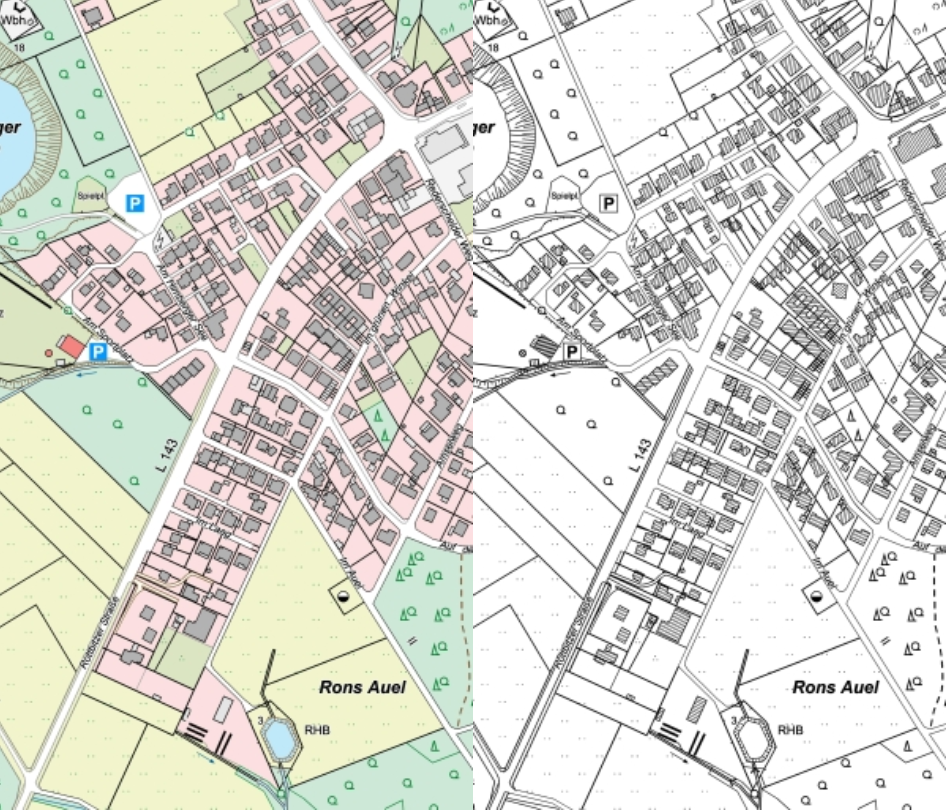
\includegraphics[width=5cm]{Medien/own/screen_example_ABK.png}
				\caption{Beispiel Ausschnitt Amtlicher Basiskarte (farbig und schwarz-weiß) \cite{web_bezreg_koeln_alkis_abk}}
				\label{fig:ABK_example}
			\end{wrapfigure}

			% 3) Beschreibung:	Format
			Die Amtlichen Basiskarten liegen in Schwarz-/Weiß- oder Farbausprägung als Raster Graphiken mit 1:5000 Maßstab für NRW unterteilt in quadratische 1 $km^2$ Kacheln mit dem Datei-Format .tiff vor. Allein für NRW ergeben sich daraus in etwa 35.000 Einzel-Kacheln respektive Dateien mit einer Größe von jeweils 74 kB in farbiger Ausprägung (ca. 7,8 MB gesamt). Das KBS ist ETRS89/UTM32 (EPSG:25832). \cite{web_download_opengeodata_nrw}
			
			% 4) Bewertung:		Eignung
			Die Amtliche Basiskarte eignet sich gegebenenfalls zur Visualisierung von lokalen Gegebenheiten, hat aber den großen Nachteil nicht vektorbasiert zu sein, sodass sie sich kaum zur Weiterverarbeitung oder zur Verknüpfung mit weiteren Datensätzen eignet. Die Menge an Dateien würde zur Reduzierung auf ein gesuchtes Areal eine Vorauswahl nach Kachel-ID erfordern. 
			
			Als Alternative zur ABK kann das Kartenmaterial des OpenStreetMap-Konsortiums dienen.

		\subsection{OpenStreetMap (OSM) Basiskarte (Vektor-Graphik)}	
			% 1) Intro: 		Wofür und von wem
			Um für Base-Layer wichtige topologische Merkmale wie Stadt- und Verkehrsinfrastruktur (u.A. Gebäude, Straßen, Schienen), landschaftliche Merkmale (z.B. Gewässer, Felder, Wälder, Wiesen) und mehr darzustellen bieten sich neben der ABK auch das OpenStreetMap Kartenwerk an. OSM ist ein 2004 gegründetes Projekt mit dem Ziel freies Kartenmaterial oder im Allgemeinen Geoinformationen zu erstellen und stellt diese Daten seit 2012 unter der \textit{Open Database Licence (ODbL) 1.0} bereit. \cite{web_osm_de}
			
			% 2a) Beschreibung: Vorbemerkung Inhalt
			Da die Daten von Freiwilligen weltweit gesammelt, überprüft und aktualisiert werden ist die Menge, Korrektheit und Genauigkeit erfasster Merkmale regional unterschiedlich und in keinster Weise rechtlich garantiert. Sowohl aus eigener Erfahrung als auch, was die Aktivität und Anzahl an Commits innerhalb der OSM-Community angeht lässt sich sagen, dass der Detailgrad innerhalb Deutschlands flächendeckend sehr hoch ist und alle der erwähnten Merkmale abdeckt. OSM-Daten finden daher auch in einer Vielzahl an Applikationen Anwendung. \cite{web_osm_de}
			
			Das OpenStreetMap-Wiki bietet eine gute Übersicht der erfassten Objekte im OSM-Datensatz und die verwendeten Tags zur Kennzeichnung bestimmter Merkmale (z.B. Straßentyp oder Typ der Landnutzung). Für eine Darstellung in QGIS bedarf es hierfür Style-Definitionen, um verschiedene Merkmale differenziert anzeigen zu können. QGIS selbst bietet hierfür keine standardmäßig verwendeten Style-Definitionen. Auch über die OSM-Webseite sind solche Styles für QGIS nicht verfügbar. \cite{web_osm_wiki}
			
			\begin{figure}[H]
				\begin{subfigure}{0.5\linewidth}
					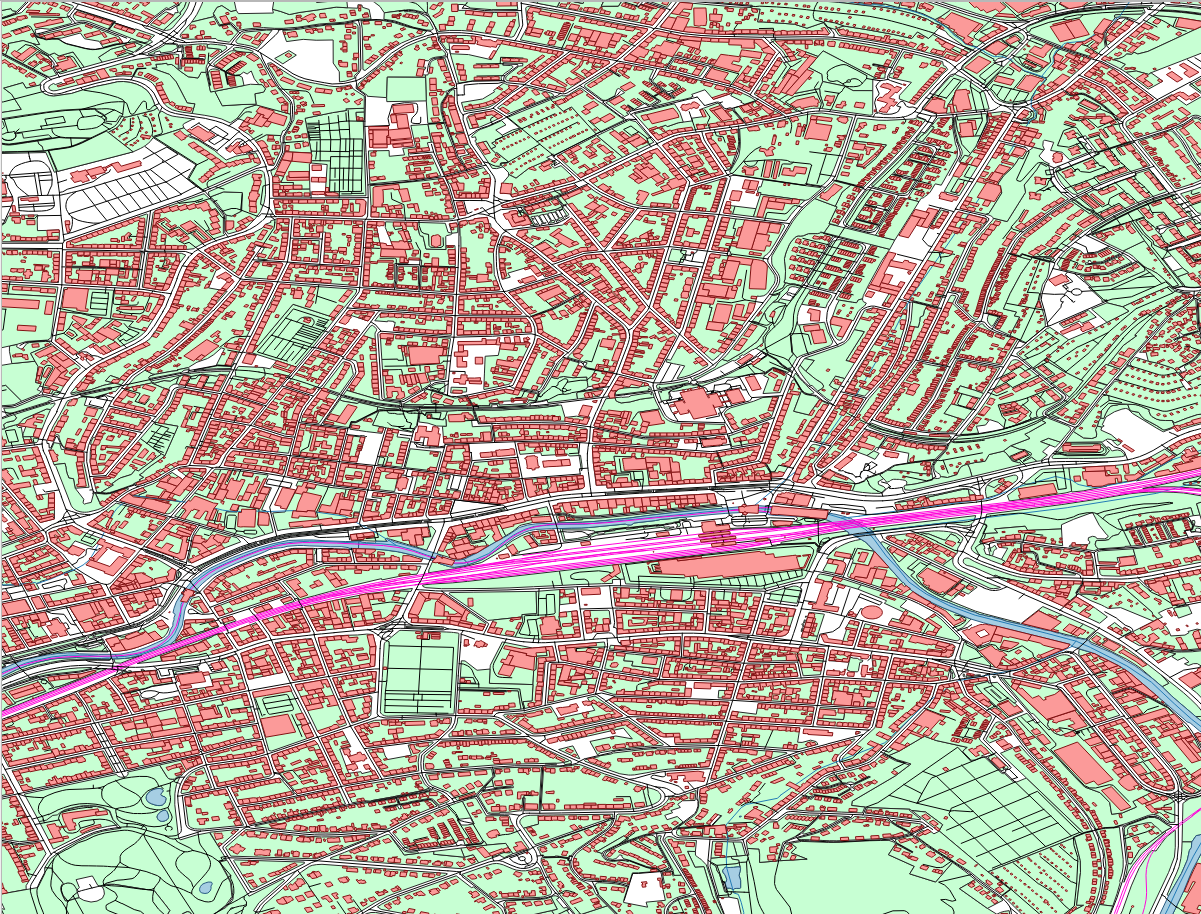
\includegraphics[width=\linewidth]{Medien/own/screen_osm_example_style_own_quick.png}
					\caption{Eigener Layer Style ("quick and dirty")}
					\label{fig:osm_example_style_own}
				\end{subfigure}
				\begin{subfigure}{0.5\linewidth}
					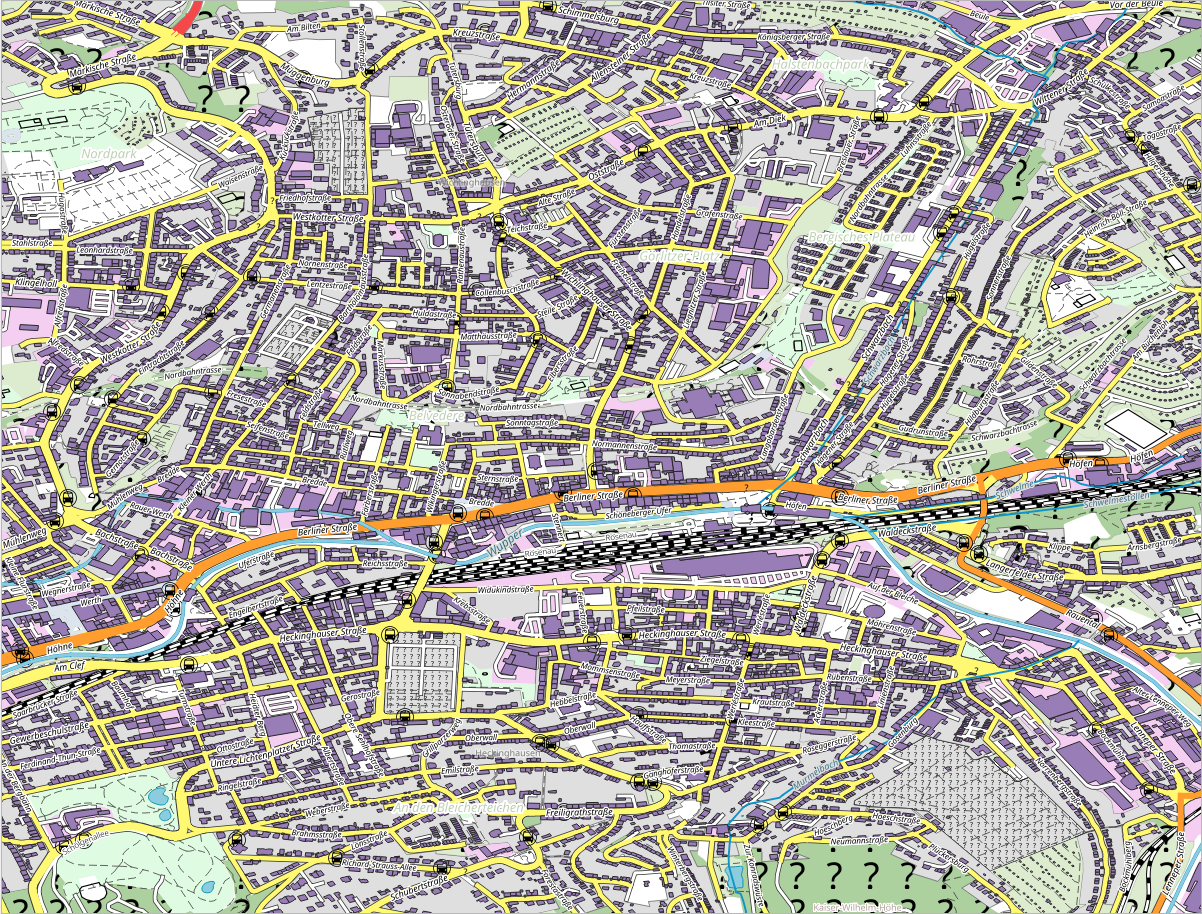
\includegraphics[width=\linewidth]{Medien/own/screen_osm_example_style_champs_libres.png}
					\caption{Style von champs-libres \cite{web_gitlab_champs_libres}}
					\label{fig:osm_example_style_champs_libres}
				\end{subfigure}
				\caption{Beispiel OSM Darstellung in unterschiedlichen QML Styles}
				\label{fig:osm_example}
			\end{figure}
			
			Als gute Basis für eine Style-Definition haben sich die OSM-Styles von champs-libres herausgestellt, insbesondere für die Darstellung von Straßenzügen nach Typ (Autobahn, Bundesstraße, Landstraße, etc.) und Gebieten nach Typ der Landnutzung (z.B. Wohn-, Industrie-, Wald-, Wiesengebiete und Tagebaue). Eine Beispiel-Darstellung eines Kartenausschnitts mit eigenen Layer-Styles (quick and dirty) und denen von champs-libres sind zum Vergleich in \autoref{fig:osm_example} gezeigt. Einige Symbole, beispielsweise bei der Anzeige von Friedhöfen (in der Abbildung am unteren Bildrand) oder Tagebauen wurden allerdings in der aktuellen Version von QGIS nicht korrekt dargestellt. Zur Korrektur bietet sich eine manuelle Nachbearbeitung in QGIS an. \cite{web_gitlab_champs_libres}

			% 2b) Beschreibung: Inhalt
			Das OSM Kartenmaterial kann entweder als sogenanntes planetfile für den gesamten Globus direkt von den Servern einer englischen Universität heruntergeladen werden oder über Drittanbietern wie z.B. der Geofabrik GmbH Karlsruhe. \cite{web_osm_de}\cite{web_geofabrik}

			% 3) Beschreibung:	Format
			Geofabrik bietet extracts des OSM planetfiles an, untergliedert nach Kontinent, Staatsgebiet und innerhalb Deutschlands weiter unterteilt in ganze Bundesländer oder den jeweiligen Regierungsbezirken (falls vorhanden). Die Daten werden komprimiert (als .osm.pbf, .shp.zip und .osm.bz2) zum Download angeboten und liegen dekomprimiert wahlweise in den Dateiformaten .osm oder .shp vor. Die Endung .pbf, .zip und .bz2 sind stehen für angewandte Komprimierungsformate. \cite{web_geofabrik}
			
			Für den Regierungsbezirk Köln ist das Shape File entpackt in etwa 1,2 GB groß, wovon knapp 700 MB allein auf Gebäude entfallen (ca. die Hälfte für die Database und die Hälfte für das .shp file). Es finden sich insgesamt 18 Layer. Die neun wichtigsten für Wärmeplanungen und im Laufe dieser Arbeit verwendeten Layer (in top-down Reihenfolge) sind \textit{osm\_buildings\_free\_1} (optional für Gebäude), \textit{osm\_railways\_free\_1} (für Schienen), \textit{osm\_roads\_free\_1} (für Straßen und Wege), \textit{osm\_landuse\_free\_1} (für Flächennutzungstypen), \textit{osm\_places\_free\_1} (z.B. für Ortsbezeichnungen), \textit{osm\_pois\_a\_free\_1}(Point of Interest Flächen, z.B. für Schulgelände oder Kläranlagen-Gelände, die nicht über das Landuse-Layer abgedeckt sind) \textit{osm\_traffic\_a\_free\_1} (z.B. für Parkflächen und -gebäude), \textit{osm\_water\_a\_free\_1} (z.B. für Seen und Teiche) und \textit{osm\_waterways\_free\_1} (für Wasserläufe). 
			
			Das KBS wird in QGIs durch die .proj Dateien automatisch erkannt und entspricht EPSG:4326.

			% 4) Bewertung:		Eignung
			Der hohe Detailgrad und die freie Lizenz machen die OSM-Karten zu einem geeigneten Basis-Kartenwerk. Da das.osm Dateiformat OSM-eigen ist und außerhalb kaum Anwendung findet und sich auch erst nach Konvertierung in QGIS nutzen lässt, bieten sich besonders die .shp Files an. Für konkrete Wärmeplanungen in einer Kommune können zur Überprüfung zusätzlich zum Beispiel registergestützte Daten wie die Hausumringe aus dem Amtlichen Ligenschafts-Kataster (ALKIS) herangezogen werden. 
		
		\subsection{Schutzgebiete der Landschaftsinformationssammlung (LINFOS) [LANUV]}
			Über die Plattform \textit{OpenGeoData.NRW} bietet das LANUV zum Download Schutzgebiete verschiedener Art als Teil der Landschaftsinformationssammlung (LINFOS) zum Download an. \cite{web_download_opengeodata_nrw}
			
			Die Schutzgebiete umfassen unter anderem FFH-, Landschaftsschutz-, Naturschutz-, Nationalpark-, Naturpark-, Vogelschutzgebiete sowie RAMSAR-Schutzgebiete für Feuchtgebiete. Nicht enthalten sind allerdings Wasserschutzgebiete. Die Vollständigkeit der Daten konnte aus Zeitgründen nicht näher untersucht werden. LINFOS ist eine unter mehreren Sammlungen von Schutzgebieten, welche über \textit{OpenGeoData.NRW} zum Download angeboten werden.
			
			Die Daten liegen alle als zip-komprimierte Shape-Files vor, wobei für jede Art von Schutzgebiet ein seperater Datensatz als Zip-Archiv vorliegt. Die Datensätze enthalten überwiegend je ein Shapefile, in manchen Fällen jedoch mehrere. Die Shapefiles sind etwas kryptisch benannt und werden mit polygon-, polyline- oder pointproved im Dateinamen gekennzeichnet.
			
			Der Datensatz wurde erst gegen Ende dieser Arbeit begutachtet und wird aus Zeitgründen nicht näher untersucht.
			
						
		\subsection{Hausumringe im Amtlichen Liegenschaftskataster-\\Informationssystem [ALKIS]}
			% 1) Intro: 		Wofür und von wem
			Die Hausumringe im ALKIS-Datensatz geben die Geometrie von über 10 Mio. Gebäudegrundrisse in NRW wieder. Sie stammen von den 53 Katasterbehörden in NRW, werden von der Bezirksregierung Köln, Geobasis NRW bereitgestellt und sind über OpenGeodata.NRW verfügbar. \cite{web_download_opengeodata_nrw}
			
			% 2) Beschreibung: Inhalt
			Der Datensatz für Hausumringe folgt dem ALKIS-Standard, welcher bundesweit einheitlich ist. Die Objekte enthalten zusätzlich zur Geometrie der Grundrisse die folgenden Attribute: Amtlicher Gemeindeschlüssel (AGS), Objektidentifikator (OI), Gebäude-/Bauwerksfunktion (GFK), Aktualitätsdatum (AKTUALITAE).Nicht enthalten sind Ausgestaltungsgeometrie und Dachform.
			
%			\url{https://www.bezreg-koeln.nrw.de/brk_internet/geobasis/liegenschaftskataster/aktuell/alkis-folgeprodukte/hausumringe/index.html}			
%			\url{https://www.bezreg-koeln.nrw.de/brk_internet/geobasis/liegenschaftskataster/aktuell/alkis-folgeprodukte/hausumringe/datenformatbeschreibung_hausumringe.pdf}\\
						
			% 3) Beschreibung:	Format
			Die Hausumringe liegen als Shape-File mit einer Größe von ca. 2,5 GB vor. Die Einträge für die Gebäude- und Bauwerksfunktion in der Database liegen codiert vor, z.B. '31001\_1000' für 'Wohngebäude'. Die Zuweisung von Codes zu Beschreibungstext ist in Form einer .xml-Datei gegeben. Insgesamt liefert diese nach eigener Auswertung 301 Definitionen für Gebäude- bzw. Bauwerksfunktionen.  \cite{web_download_alkis_gebaeudefunktion_code_definition}
			
			Das KBS ist EPSG:25832 (ETRS89/UTM32)		
			
			% 4) Bewertung:		Eignung
			Die Hausumringe des ALKIS eignen sich zur Darstellung von Gebäuden, optional mit Gebäudefunktions-Bezeichnungen oder Einfärbung je nach Gebäudefunktion. Im Zuge dieser Arbeit verwendet wurden nur die ALKIS-Daten für NRW. Seit Dezember 2015 ist das ALKIS laut Arbeitsgemeinschaft der Vermessungsverwaltungen der Länder der Bundesrepublik Deutschland (AdV) aber in allen Bundesländern eingeführt, wodurch die Hausumringdaten diesen Formats bundesweit verfügbar sind. \cite{web_alkis_adv}
		
		%\subsection{Grundrissdaten im Amtlichen Liegenschaftskataster [ALKIS]}\\
			
		%	Städteweise in NRW \text{gru\_<ARS>\_<Stadtname>\_EPSG25832\_NAS.zip}\\
			
		%	\url{https://www.opengeodata.nrw.de/produkte/geobasis/lk/akt/gru_xml/}\\
					
		\subsection{Gebäude- und Wohnungsbestand [Zensus2011]}
		\label{sec:Daten:Datensatz:Zensus2011}
			% Was ist der Zensus 2011
			Im Zuge der Volkszählung 2011 in der Europäischen Uninion wurde in Deutschland der Zensus 2011 zur Datenerhebung durchgeführt. Gesetzliche Basis in Deutschland für die registergestützte Datenerhebung ist das bundesdeutsche Zensusgesetz 2011 mit welcher die EG-Verordnung 763/2008 umgesetzt wurde, welche eine Datenerhebung alle 10 Jahre vorsieht. Das Gesetz definiert den Stichtag (9. Mai 2011), die Erhebungsmerkmale (u.A. Alter, Geschlecht, Schulabschluss, Wohnfläche, etc.) und die Auskunftspflichtigen. Im Zuge des Zensus wurden neben Daten zur Population auch umfassend Daten zum Gebäude- und Wohnungsbestand erhoben.
			
			\subsubsection{Potentieller Nutzen und Vollständigkeit}
				% Potentieller Nutzen für Wärmeplanungen
				Für Wärmeplanungen können die Daten zum Gebäude- und Wohnungsbestand zur Bestandsaufnahme nützlich sein. Die Anzahl, Größe und das Alter von Wohnungen bietet sich als Indikator für Sanierungspotential von Gebäuden an. Bereits durchgeführte Sanierungsarbeiten werden zwar nicht zentral erfasst, aber in Gebieten mit einer hohen Dichte von Altbauten und Population ist sowohl das Sanierungspotential als auch i.d.R. der spezifische Wärmeverbrauch je Wohnfläche größer. 
				
				% Aktualität und räumliche Auflösung
				Die Daten des Zensus 2011 stellen zum Zeitpunkt dieser Arbeit die aktuelle Zensus-Datenbasis, da die Ergebnisse der Folge-Zählung Zensus 2022 vorraussichtlich erst 2023 veröffentlicht werden. Neben dem umfangreichen Datenangebot für aggregierte Werte für Kommunen, Kreise, Länder und Bund bietet die Zensus-Datenbank auch gitterzellenbasierte Datensätze für Gebäude und Wohnungen an, welche in einem INSPIRE-kompatiblen 100m x 100m Raster vorliegen. Letztere sollen aufgrund ihrer höheren Auflösung näher untersucht werden. 
				
				% Räumliche Abdeckung und geheimhaltungsbedingte Abweichung
				Die Zensus-Datenbank bietet in Deutschland hinsichtlich Gebäudebestand die umfangreichste und flächendeckendste Datenbasis, da sie gesamte Bundesgebiet abdeckt. Aus Datenschutzgründen wurden die originalen Ergebnisse des Zensus geheim gehalten. Die Genauigkeit von aggregierten Werten, Verhältniszahlen, Anteilen und Durschnittswerten ist davon nicht betroffen, da diese aus den originären Werten abgeleitet wurden. Für die veröffentlichten Raster-Werte ist anzumerken, dass diese aufgrund der angewandten datenverändernden Verfahren zur statistischen Geheimhaltung bei zu geringen Werten nur eingeschränkt verlässlich sind. Das Statistische Bundesamt gibt einen Grenzwert von etwa 10 und weniger an, ab wann das Risiko relativer Abweichungen von mehr als 50 Prozent vom tatsächlichen Wert besteht. Hierfür enthält der Datensatz zu jedem Eintrag eine Geheimhaltungskennzeichnung, welche angibt ob es vor und nach Geheimhaltung keine bis geringe, starke oder inakzeptable Abweichungen ergeben. Gitterzellen mit nur einer Person werden zudem wie Gitterzellen ohne Person klassifiziert und Gitterzellen mit zwei Personen wie Gitterzellen mit 3 Personen. 
				
				Da geheimhaltungsbedingte Abweichungen nur bei niedrigen Raster-Werten auftreten und auch nur je Gitterzelle, für Wärmeplanungen i.d.R. aber Gebiete mit hoher Populations- und Wohnungsdichte relevant sind und zudem größere Gebiete betrachtet werden, in welchen die Abweichungen sich im Mittel wieder zum Teil ausgleichen, wird im Zuge dieser Arbeit die Genauigkeit und Vollständigkeit diesbezüglich als hinreichend erachtet.
				
			% Vergleich Mikrozensus
		
			\subsubsection{Inhalt gitterzellbasierter Zensus-Daten (Gebäude, Wohnungen)}
			
				In der gebündelten Datensatzbeschreibung der Statistischen Ämter des Bundes und der Länder für die beiden Zensus 2011 Datensätze für Gebäude und Wohnungen wird aufgeführt, welche Merkmale erfasst werden und welche Ausprägungen diese haben können. Zu den Merkmalen gehören die Gesamtzahl, Gebäudeart, Gebäudebauweise, Gebäudegröße, Wohneigentum, Eigentum, Nutzung nach Belegung durch Haushalt, Heiztyp, Wohnfläche, Baujahr, Raumanzahl und Zahl der Wohnungen. Zum Beispiel gibt es für das Merkmal \textit{Heiztyp} u.A. die Ausprägungen \textit{Fernheizung (Fernwärme)}, \textit{Etagenheizung} und \textit{Zentralheizung} und für das Merkmal Baujahr entsprechen die Ausprägungen den im Mikrozensus verwendeten Baualters-Klassen, z.B. \textit{Vor 1919}, \textit{1919 - 1948}, usw.. Manche Merkmale wie z.B. die Wohnungsgröße finden nur im Wohnungs-Datensatz Anwendung.
				
				Die zu jedem Merkmal erfassten Ausprägungen, sind sowohl als Zahlencode als auch in Textform (deskriptiv) hinterlegt. \autoref{tab:Zensus2011_Merkmale} zeigt beispielhaft eine Liste an Merkmalen und zugehörigen Ausprägungen für den Wohnungs-Datensatz, welche zur Bestandsaufnahme betrachtet werden können. 
				
				\begin{table}[H]
					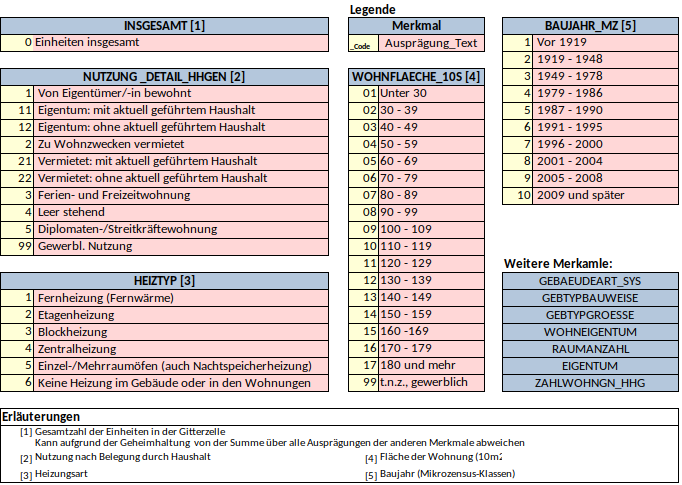
\includegraphics[width=1.00\textwidth]{Medien/tables/Zensus2011_Wohn_Geb_Merkmalev3.png}
					\caption{Liste von Merkmalen und Ausprägungen im Zensus 2011 Datensatz zu Wohnungen und Gebäude im 100m Gitterraster}
					\label{tab:Zensus2011_Merkmale}
				\end{table}
			
				Aus den Datensätzen lässt sich direkt entnehmen, wie viele Gebäude oder Wohnungen beispielsweise über eine Zentralheizung verfügen, wie viele Wohnungen einer bestimmten Wohnflächen-Kategorie oder einer Altersklasse vorhanden sind, ebenso die Leerstandsquote. Die Anzahl wie oft Ausprägungen von Merkmalen auftreten wird dabei isoliert von einander angegeben. Eine direkte Verknüpfung von Merkmalen lassen die Datensätze im Allgemeinen nicht zu. Wenn es beispielsweise Wohnungen gibt mit unterschiedlichen Heiztypen und die Wohnungen aus verschiedenen Altersklassen stammen, lässt sich nicht ableiten, wie oft, welcher Heiztyp in Wohnungen einer bestimmten Altersklasse vorhanden ist.
			
			\subsubsection{Format gitterzellenbasierter Zensus-Daten (Gebäude, Wohnungen)}
			\label{sec:Daten:Datensatz:Zensus2011:Aufbau}
			% Aufbau der von den statistischen Ämtern von Bund und Ländern veröffentlichten Daten 
			% INSPIRE Gitter-kompatibel
			
				Beide Datensätze sind in tabellarischer Form als csv Datei verfügbar mit 8 Spalten für einen Index, die Gitter-ID (in zwei Schreibweisen), die Ausprägung (als Code und als Text), die Anzahl und die Qualitätsgüte. 
				
				Der Index ist eine eindeutige Identifikationsnummer, die Gitter-ID gibt die Koordinaten des südwestlichen Eckpunkts einer Gitterzelle an. Merkmal und Ausprägung geben in jeder Zeile an, welche Größe in der Spalte Anzahl quantitativ erfasst wurde. Die Qualitätsgüte gibt an, ob die angegebene Anzahl aufgrund der angewandten geheimhaltungsbedingten datenverändernden Verfahren nicht bis wenig (0), stark (1) oder inakzeptabel (2) vom ursprünglichen Wert abweicht. 
			
				\begin{table}[H]
					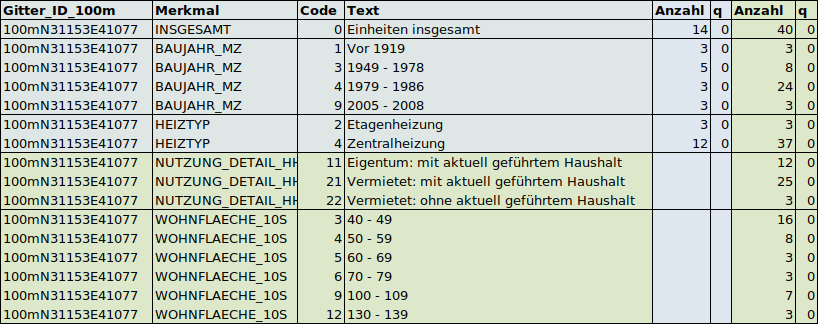
\includegraphics[width=1.00\textwidth]{Medien/tables/Zensus_2011_Wohn_Geb_Bsp_Gitterzelle.png}
					\caption{Darstellung der Daten einer Gitterzellen aus dem Zensus-Datensatz für Gebäude und Wohnungen. Spalten für Zeilen-ID und Gitter\_ID\_100m\_neu sowie Zeilen bestimmter Merkmale entfernt. \\ 
					(Blaugrün mit Blau ohne Grün: Gebäudedatensatz, Blaugrün mit Grün ohne Blau: Wohnungsdatensatz)\\
					Geänderte Spaltenbezeichnungen: Ausprägung\_Code: Code, Ausprägung\_Text: Text, Anzahl\_q: q}
					\label{tab:Zensus2011_Wohn_Geb_Bsp_Gitterzelle}
				\end{table}
			
				\autoref{tab:Zensus2011_Wohn_Geb_Bsp_Gitterzelle} zeigt exemplarisch die Werte einiger Merkmale beider Datensätze für die selbe Gitterzelle zum Vergleich. Abzulesen ist beispielsweise, wie viele Wohnungen einer bestimmten Altersklasse auf wie viel Gebäude aufgeteilt sind. Ebenso lässt sich ablesen, dass 3 der 40 Wohnungen derzeit unbewohnt sind. Bei Betrachtung der Heiztyp-Angaben zeigt sich, dass sich 37 mit Zentral- und 3 mit Etagenheizung beheizte Wohnungen auf je 12 bzw. 3 Gebäude aufteilen. Von den 3 Gebäuden mit Etagenheizung müssten 2 über unbeheizte Etagen und das dritte zusätzlich über eine Zentralheizung verfügen. Bemerkenswert ist zudem noch, dass in dieser Gitterzelle zwar alle 14 Gebäude, aber nur 38 der 40 Wohnungen mit Altersklasse erfasst sind. Dies ließe sich nur durch geheimhaltungsbedingte Nicht-Erfassung erklären, wenn beide Wohnungen aus zwei von einander und von allen anderen Wohnungen unterschiedlichen Altersklassen stammen, z.B. durch Zu- bzw. Anbau oder durch Ungenauigkeit der Daten.  
				
				Die Gitter-Geometrie ist INSPIRE-kompatibel mit KBS(CRS) ETRS89-LAEA Europe - EPSG:3035 und die Daten liegen als .csv-Dateien mit UTF-8 Codierung in einer Größe von 2,0 GB (für Gebäude) bzw. 4,3 GB (für Wohnungen) vor. 
	
			\subsubsection{Bewertung auf Eignung}
				
				Die Daten des Zensus zum Wohnungs- und Gebäudebestand besitzen einen hohen Grad an Repräsentativität, bieten inhaltlich relevante Informationen für Bestandsaufnahmen durch die Erfassung von Bau-Altersklassen, Wohnflächengrößen, Heiztypen und Nutzungsart (inkl. Leerstandsquote), decken räumlich das gesamte deutsche Bundesgebiet ab, besitzen eine relativ hohe räumlichen wie inhaltliche Auflösung mit (100 m x 100 m) Gitterzellen und der vergleichsweise feinen Staffelung bezüglich Wohnungsgröße und Altersklassen sowie relativ hohe Aktualität mit Stand der Daten von 2011. 
				
				% Schwierigkeit Informationen aus Daten abzuleiten wegen datenschutzbedingter Anonymisierung
				Die Schwierigkeit bei der Auswertung der Zensus2011 Daten zu Wärmeplanungszwecken ergibt sich aus dem Umstand, dass die untersuchten Merkmale zwar gebäude- bzw. wohnungsscharf erhoben wurden, aber aus Datenschutzgründen nicht in vollem Umfang merkmalsverknüpft in dieser Auflösung öffentlich verfügbar sind. Die erfassten Merkmale spiegeln somit energetische Einzelaspekte (wie z.B. Altersklassen und Größe), lassen sich aber nicht direkt zu gesamt-energetischen Bewertungen zusammenfügen.
				
				Eine Verschmelzung mit anderen Datensätzen wie z.B. über die Häufigkeit verschiedener Dämmstandards je Altersklassen ist zwar möglich, allerdings ist zu beachten, dass solche Synthese-Datensätze einer statistischen Ungenauigkeit unterliegen, was mit einem zusätzlichen Unsicherheits-Faktor zu berücksichtigen wäre. Zudem entstünden fiktive Gebäude bzw. Wohnungen, die nicht unbedingt die realen Verhältnisse widerspiegeln. 
				
				Auf diese Problematik, was die begrenzte Verknüpfbarkeit einzelner für sich genommen valider und statistisch belastbarer Informationen angeht wird auch in anderen Untersuchungen zum deutschen Wohnunggebäudebestand hingewiesen. Vergleich [Cischinsky, Diefenbach 2018]
				
				Dennoch Stellen die Zensus-Daten zum Gebäude und Wohnungsbestand für sich bereits wertvolle Informationen für Wärmeplanungen bereit. Größenbedingt ist zur besseren Verarbeitbarkeit zum Einsatz in Wärmeplanungen eine Reduktion der Datensätze auf eine gewünschte Region und zu untersuchende Merkmale angeraten, was beim vorliegenden Dateiformat mit überschaubarem Arbeitsaufwand machbar scheint.
		
		\subsection{INSPIRE Daten und Dienste [BKG]}
			Die Direktive Infrastructure for spatial information in Europe (INSPIRE) der Europäischen Union zielt darauf ab eine Infrastruktur für Geodaten zu erstellen. INSPIRE soll das Teilen von umweltbezogener Geodaten zwischen Organisationen des öffentlichen Sektors ermöglichen, den öffentlichen Zugang zu Geodaten in ganz Europa erleichtern und grenzüberschreitende Strategie-Entwicklungen unterstützen. \cite{web_inspire}
			
			Das Bundesamt für Kartographie und Geodäsie (BKG) bietet auf deren Website einige INSPIRE-konforme Dienste an. Zu diesem INSPIRE-Angebot gehören beispielsweise Geographische Bezeichnungen, Gewässernetze, Bodenbedeckung, Schutzgebiete, Transportnetze, Verwaltungseinheiten, Höhenmodelle und statistische Einheiten. Die angebotenen Dienste lassen sich via URL in ein GIS einbinden. Allerdings werden die Daten nicht direkt für eine offline-Nutzung zum Download angeboten. In der Open Data Sektion finden sich weitere Datensätze, u.a. aufbereitete Satellitenfotos als Mosaik aus dem Erdbeobachtungsprogramm Copernicus (Sentinel-2, L1C und L2A) für die Bundesrepublik Deutschlands, wobei die Satelittenfotos vom BKG ebenfalls nicht direkt zum Download angeboten werden. Die genannten Daten wurden aufgrund der nicht direkten offline Bearbeitbarkeit in dieser Arbeit außer Acht gelassen. \cite{web_inspire_bkg}
			
			Neben den anderen Diensten enthält die Seite des BKG auch eine Sektion für ein INSPIRE-konformes Geographisches Gittersystem. Dieses definiert laut BKG kein eigenständiges Datenmodell, sondern beschreibt Festlegungen zur Georeferenzierung von Geodaten. Das Gittermodell findet beispielsweise Anwendung Datensatz des Zensus 2011 und bietet sich Analyse und Darstellung statistischer Sachverhalte an. \cite{web_inspire_bkg}
			
			In der Dokumentation zu Geographischen Gittersystemen des BKG findet sich die folgende Beschreibung: \frqq Die europäische Initiative zum Aufbau einer Geodateninfrastruktur INSPIRE definiert im Dokument D2.8.I.2
			Data Specification on Geographical Grid Systems – Technical Guidelines europaweit einheitliche Geographische Gitter. Ein grundlegender Parameter ist dabei das verwendete Georeferenzsystem. INSPIRE unterscheidet:\\
			\quad Equal Area Grids – auf der Grundlage von ETRS89-LAEA (EPSG:3035)\\
			\quad Zoned Geographic Grids – auf der Grundlage von ETRS89-GRS80 (EPSG::4258) [sic]\\
			Für den Bereich Deutschlands sind Equal Area Grids von Interesse. Diese bilden gemäß INSPIRE ein hierarchisches System mit Gitterauflösungen von 1 m, 10 m, 100 m, 1 km, 10 km, 100 km.\flqq \cite{web_inspire_bkg_gittersysteme}
				
			Aus diesem Grund wird zur Darstellung in QGIS im Zuge dieser Arbeit das KBS ETRS89-LAEA (EPSG:3035) verwendet. 
			
			In der Dokumentation werden zudem einheitliche Bezeichnungen für Gitterzellen definiert \cite{web_inspire_bkg_gittersysteme}. Die Gitterzellen-Codierung für die Auflösungen 100~m und 1~km sehen dabei wie folgt aus: 
			
			Größe = 1~km: Ersten 4 Stellen der Koordinaten Ymin und Xmin
			
			Größe = 100~m: Ersten 5 Stellen der Koordinaten Ymin und Xmin
			
			Zellen-ID = <Größe>"N"<Ymin>"E"<Xmin>, z.B. "1kmN3121E4112" oder "100mN31210E41120"
		
		\subsection{Energie-Erzeugungs-Anlagen-Standorte NRW [LANUV]}
			% 1) Intro: 		Wofür
			Das LANUV NRW stellt über OpenGeodata.NRW einen großen Datensatz für Energie-Erzeugungsanlagen (Strom und Wärme) mit Standorten für NRW zur Verfügung. Zudem enthalten sind zusätzliche Informationen wie Strom- und Wärmeverbräuche für Gemeinden. Der Datensatz kann für die Bestandsaufnahme zur örtlichen Darstellung von Anlagen sowie der gebietsweise aggregierten installierten Leistungen und Anlagenzahl je Energieträger genutzt werden. \cite{web_download_opengeodata_nrw}
			
			% 2) Vorbemerkung
			Eine direkt verfügbare Dokumentation zum Datensatz fand sich nicht, allerdings sind die Daten größtenteils selbsterklärend. Der Datensatz liegt sowohl als Geodatabase (.gdb) mit 555 MB als auch in mehreren Excel-Files (.xlsx) vor, wobei die Inhalte nicht vollständig deckungsgleich sind. \\
			
			% 2a) Inhalt: Standorte
			\textbf{Inhalts-Beschreibung: Excel-Datei zu Anlagen-Standorten:}\\
			Ein Excel-File enthält die Standorte von Anlagen, wobei diese nach Energieträger bzw. Art der Anlage unterteilt in jeweils seperaten Sheets abgespeichert sind. Zu den Energieträgerarten bzw. Anlagentypen gehören: Biomasse, Deponiegas, Grubengas, Klärgas, PV-Freifläche, Wasserkraft, Wind, WEA in Planung, WEA stillgelegt, E-Tankstellen, Braunkohle, Steinkohle, Erdgas, Mineralöl, Sonstige (z.B. Kondensationsmaschinen und Gegendruckmaschinen), Müllverbrennungsanlagen (MVA), Grubenwasserschächte, Grubenwasserhaltungen, Grubenwasserprojekte, Indsturielle-Abwärme und KWK-relevante-Industriestandorte. Aufgrund der Vielzahl unterschiedlicher Anlagentypen ergeben sich auch unterschiedliche Attributszuweisungen je Typ.
			
			Zu den gelisteten Attributen (Spaltenbezeichnungen) je Anlage (Zeileneinträge) gehören im Allgemeinen eine LANUV-ID, zugehörige Verwaltungsgebiete, AGS, die PLZ, Gemeindenamen, Geo-Koordinaten in UTM32-Format, Status (z.B. 'in Betrieb'), Inbetriebnahme-Jahr, Leistung in kW, gegebenenfalls auch Leistung seperat für Strom und Wärme in kW, Zahl der Einheiten und KWK (z.B. 'Ja', 'Nein', 'Nein, Ja', 'Ja, Nein') und der Stand der Daten. In manchen Fällen ist zusätzlich zur LANUV-ID auch eine korrespondierende MaStR-ID gegeben.
			
			Zusätzliche Attribute gibt es z.B. für Windkraftanlagen. Hier werden auch, Hersteller, Anlagentyp, Durchmesser, Nabenhöhe und Höhe insgesamt gelistet. Etwas andere Attribute gibt es auch für Erzeugungs-Anlagen mit fossilen Brennstoffen (Braunkohle, Steinkohle, Erdgas, Mineralöl). Hier wird die elektrische Leistung in MW (brutto und netto) angegeben, ob Wärmeauskopplung gegeben ist und die CO2-Emissionen, gegebenenfalls auch weitere verwendete Brennstoffe und die Anzahl der Kraftwerks-Blöcke. Auch die Einträge sind nicht immer einheitlich bzw. unterscheiden sich vom Informationsgehalt. Bei MVA ist unter Wärmeauskopplung teilweise nichts vermerkt (Datenlücke) oder nur 'ja' bzw. 'nein', teilweise auch der Wärmeertrag für Fernwärme oder für Prozessdampf in MWh. Die Werte sind dann als string hinterlegt z.B. in der Form: 'Fernwärme: 2.069 MWh (2021)' oder 'Prozessdampf: 449.649 MWh (2021)'. Ähnliches gilt für den Stromertrag von MVA. Die Werte reichen von '' (leer) über 'ja', 'nein' zu bspw. 'Stromabgabe: 85.406 MWh (2021)'. \\
			
			\textbf{Inhalts-Beschreibung: Excel-Datei zu Anlagen-Standorten, Limitierungen:}\\
			In der Excel-Datei sind keine Informationen zu PV-Anlagen auf Dächern enthalten, da diese laut enthaltener Vorbemerkung zahlenmäßig mit mehr als 315.000 Anlagen zu umfangreich seien. 
			
			Zudem werden aus Datenschutzgründen Anlagen mit kleiner 30 kW nicht mit exaktem Standort angegeben. Die Koordinaten zeigen in diesem Fall auf die Mitte der Postleitzahl. Laut LANUV sind für manche Anlagen einzelne Anlagenattribute nicht bekannt, weshalb der Datenbestand Lücken zeigt. 
			
			Die Daten zu Industrieller Abwärme aus der Potentialstudie des LANUV liegen nur gemeindescharf vor und sind recht unvollständig. Die potentielle Leistung und potentielle Abwärme wird als Bereich angegeben, in der Regel mit Faktor $10^1$, $10^2$ oder $10^3$ zwischen Minimum und Maximum. 
			
			Die vorliegenden Daten im Sheet 'KWK\_relevante\_Industriestandort' aus der zugehörigen Potentialstudie des LANUV enthalten als Attribut neben einer Objekt-ID, dem Unternehmensnamen, Geokoordinaten und der Aktualität der Daten lediglich einen Eintrag für den Prozesswärmebedarf in $\left[GWh/a\right]$.\\
			
			% 2b) Inhalt: Aggregiert Wärme
			\textbf{Inhalts-Beschreibung: Excel-Datei zu aggregierten Wärme-Werten:}\\
			Eine weitere Excel-Datei enthält aggregierte Werte zur installierten Wärmeerzeugungs-Leistung verschiedener Anlagentypen unterteilt nach den Verwaltungsgebiets-Größen Bundesland NRW, Regierungsbezirke, Planungsregionen, Kreise und Gemeinden je Sheet. 
			
			Zusätzlich finden sich hier Raumwärme- und Warmwasser- (zusammengefasst), Prozesswärme- (<500 °C) und Raumkälte-Bedarfe sowohl aktuell als auch prognostiziert für die Jahre 2030, 2040 und 2050. Für den Raumkälte-Bedarf gibt es allerdings keine Prognosen für die Jahre 2030 und 2040. Daten zu jährlichen Wärmeerträgen gibt es für die Energieträger Deponiegas, Grubengas, Klärgas, Solarthermie, Geothermie, MVA, Warmes Grubenwasser, Industrielle Abwärme, KWK. Diese gibt es nicht für die Energieträger Biomasse, Braunkohle, Steinkohle, Erdgas, Mineralöl und sonstige Kraftwerke. \\
			
			% 2c) Inhalt: Aggregiert Strom
			\textbf{Inhalts-Beschreibung: Excel-Datei zu aggregierten Strom-Werten:}\\
			Die letzte Excel-Datei enthält aggregierte Werte zur Stromerzeugung und ist ähnlich aufgebaut wie die Excel-Tabellen für aggregierte Werte der Wärmeerzeugung. Neben einem Übersichts-Sheet für NRW gibt es für jede Verwaltungsgebietsgröße (NRW, RBZ, Planungsregionen, Kreise, Gemeinden) zwei Sheets, einmal für alle erneuerbaren und einmal für alle konventionellen Energieträger.\\ 
			
			% 2) Beschreibung: 	Inhalt
			% 3) Beschreibung:	Format
			\textbf{Format und Aufbau der Geodatabase:}\\
			Die Geodatabase hat das KBS EPSG:25832 und enthält insgesamt 325 einzelne Layer. Diese sind non-hierarchisch abgespeichert, lassen sich anhand der Layernamen aber gruppieren bzw. einteilen, zudem geben die Layernamen recht genau den Inhalt wieder.\\
			
			\textbf{Format der Geodatabase: Layernamen-Aufbau:}\\
			Zur Einordnung der Layer, werden diese hier nach Art und Ausprägung, gegebenenfalls nach Ausführung unterteilt. Die Art wird durch den ersten Abschnitt im Layernamen (bis zum ersten Unterstrich) gekennzeichnet. Als Ausprägung gilt der zweite Teil des Layernamen (nach dem ersten Unterstrich) exclusive einer potentiellen räumlichen Einteilung (Ausführung), für welche Werte aggregiert wurden. Veranschaulicht wird diese Einteilung an den folgenden zwei Beispielen:\\
			
			Beispiel Layername (mit Ausführung) = 'Biomasse\_Installierte\_Leistung\_RegBez' \\
			$\rightarrow$ Art = 'Biomasse', Ausprägung = 'Installierte\_Leistung', Ausführung = 'RegBez'. \\
			
			Beispiel Layername (ohne Ausführung) = 'Biomasse\_Standorte'\\
			$\rightarrow$ Art = 'Biomasse', Ausprägung = 'Standorte'\\
			
			\textbf{Inhalt der Geodatabase: Layernamen-Arten:}\\
			An Arten gibt es 22, wovon 18 für Energie-Erzeugungsanlagen stehen. Ausnahmen sind die vier Layer mit Art: 'z4', 'z6', 'Statistik' und 'StromInfra'. Die Art 'z4' umfasst ein Layer für Freileitungen und 'z6' eines für Kreise. Die Art 'Statistik' beinhaltet die beiden Ausprägungen 'Stromverbrauch' und 'Anteil\_EE\_am\_Stromverbrauch'. 
			
			Die Art 'StromInfra' beinhaltet die Ausprägungen für E-Tankstellen (Grünström, Gesamt) und Großspeicher. Die anderen 18 Arten stehen für verschiedene Energieträger, wobei es für PV und Wind jeweils 3 Arten gibt: 'PVDach','PVFrei', 'PVGesamt', 'Wind$[$Bb$]$etrieb', 'WindGen' und 'Windstill'. Anmerkung: Wegen Typo einmal 'WindBetrieb' und 18 mal 'Windbetrieb'.
			
			Von den 13 Energieträgern insgesamt werden für Wärmeplanungen als direkt relevant die zehn Arten Biomasse, Braunkohle, Deponiegas, Erdgas, Grubengas, Klärgas, Mineralöl, Müllverbrennung, sonstigeKW, Steinkohle eingeordnet, als indirekt relevant die sieben Arten für die drei Energieträger Wind, Wasser und PV. \\
			
			\textbf{Inhalt der Geodatabase: Layernamen-Ausprägungen und -Ausführung:}\\
			Für die Layer nach Energieträgern gibt es die Ausprägungen 'Standorte', 'Anzahl\_an\_Anlagen' und 'Installierte\_Leistung', letztere beide in den Ausführungen 'NRW', 'RegBez', 'Planungs$[$Rr$]$eg', 'Kreise', 'RheinRevier', 'Gemeinde(n)'. Für die Arten 'Biomasse', 'Deponiegas', 'Grubengas', 'Klärgas', 'Müllverbrennung, 'PV(...)', Wasserkraft und 'Wind(...)' gibt es noch die Ausprägung 'Stromertrag' mit den gleichen Ausführungen.\\
					
			% 4) Bewertung:		Eignung
			\textbf{Bewertung auf Eignung:}\\
			Die Standort-Daten der Wärme- und Stromerzeugungsanlagen der Geodatabase bieten sich sowohl zur kartographischen Darstellung als auch zur räumlichen Aggregation der installierten Leistung in Sub-Areale von Gemeinden an. 
			
			Die Industrielle-Abwärme-Standorte und KWK-relevante Standorte, welche nur im Excel-Dataset vorliegen, bieten sich zur Konvertierung in ein Vektorformat an, um diese zusätzlich zu berücksichtigen. 
		
		
			%----------
			%Daten im xlsx-Format (Excel) mit mehreren Sheets je Datei.\\
			%Anleitung zum Formatieren nach csv:\\
			%mit ssconvert command aus dem package gnumeric im Terminal (Linux)\\
			%ssconvert Version »1.12.46« datadir := »/usr/share/gnumeric/1.12.46« libdir := »/usr/lib/gnumeric/1.12.46«\\
			%ssconvert -S file.xls "	
		
		
		\subsection{Enerige-Erzeugungs-Anlagen-Standorte BRD [MaStR]}
			Da der Fokus dieser Arbeit auf die Aufbereitung von Daten für NRW liegt, sei hier nur angemerkt, dass bundesweite Daten zu Energie-Erzeugungs-Anlagen wie deren Art, Standort und installierte Leistung im Marktstammdatenregister (MaStR) vorliegen.  \cite{web_mastr}
			
		\subsection{Raumwärmebedarfs-Modell NRW [LANUV]}
			% 1) Intro: Wofür, Was
			Im Rahmen der 2015 vom LANUV durchgeführten Potentialstudie zum Geothermie-Potential in NRW hat das LANUV einen Raumwärmebedarfs-Modell (RWB-Modell) entwickelt, welches über OpenGeodata.NRW zum Download angeboten wird. Das RWB-Modell ist ebenfalls im Web-Tool \textit{energieatlas.nrw} integriert. \cite{lanuv_potentialstudie_geothermie} \cite{web_download_opengeodata_nrw} \cite{web_energieatlas} \\
			
			% 2) Inhalt
			\textbf{Inhalt:}\\
			Das Modell umfasst zwei Datensätze. Der erste enthält Hausumringe mit modellierten Wärmebedarfen je Hausumring, der zweite enthält Wärmeliniendichten mit Wärmebedarfen je Straßenzug. Die modellierten Wärmebedarfe umfassen dabei die Bedarfe für Raumwärme und Warmwasser und sind jeweils absolut (je Hausumring bzw. Straßenzug) als auch relativ (je Flächeneinheit je Jahr bezogen auf die Nutzfläche bzw. je Längeneinheit je Jahr bezogen auf die Straßenlänge) angegeben. Die Berechnungsgrundlage ist beschrieben in \cite{lanuv_potentialstudie_geothermie}.
			
			Für die Hausumringe sind zudem zahlreiche weitere Angaben enthalten wie beispielsweise ein Objektschlüssel, die Gebäudehöhe, die Jahres-Mitteltemperatur, eine Gebäudeklasse, das Gebäudevolumen, ein Gebäudetyp, der AGS, die ID der Gitterzelle der INSPIRE-Raster, der Gemeindename, der Kreisname sowie ein eindeutiger Objekt-Identifikator und eine ID des zugehörigen Straßenabschnitts. AGS, Gemeindename und Kreisname beziehen sich auf die Gemeinde bzw. den Kreis, in welcher der Hausumring steht.
			
			Der Objektschlüssel ist laut Datensatz-Beschreibung in der im Download enthaltenen .pdf unterschiedlich für Bestand (ALKIS) und Neubau (LoD1). Die Gebäudeklasse bezeichnet eine Klassifikation der Gebäude nach Heizbedarf. Angegeben sind die Klassen null bis vier für nicht beheizte Gebäude (unabhängig des Objektschlüssels), Wohngebäude (nicht weiter differenziert), Nichtwohngebäude mit normalem, geringerem oder erhöhtem spezifischen Raumwärmebedarf. Der Gebäudetyp bezeichnet einen Typ für Wohngebäude wie Einfamilienhaus/Doppelhaushälfte (EFH/DHH), Reihenhaus (RH), Mehrfamilienhaus (MFH), Groß-Mehrfamilienhaus (GMFH) oder Hochhaus (HH). Die ID der Gitterzelle der INSPIRE-Raster ist für 100m-Raster angegeben, welche in dieser Form auch in den Zensus-Datensätzen Verwendung finden.
			
			Die Bezeichnung \textit{LoD1} beim Objektschlüssel bezieht sich auf 3D-Gebäudemodelle mit \textit{Level of Detail 1}. \textit{LoD1}- und \textit{LoD2} Modelle für NRW werden beispielsweise von der Bezirksregierung Köln angeboten. Für NRW sind diese mit Stand April 2023 flächendeckend verfügbar. \cite{web_lod1_nrw} \\
			
			% 3) Format
			\textbf{Format:}\\
			Die Daten für das RWB-Modell des LANUV liegen zum Einen als Geodatabase für ganz NRW vor, zum Anderen als einzelne Shape-Files für die digitalen Verwaltungsgebiete aller Gemeinden NRWs vor. Die Daten werden jeweils in komprimierter Form (.zip-Archiv) zum Download angeboten. Die Geodatabase für NRW bedarf dabei eines Speicherplatzes von 1,5~GB in komprimierter Form. Das verwendete KBS ist ETRS 89 / UTM Zone 32N (EPSG:25832).\\
			
			% 4) Eignung 
			\textbf{Eignung:}\\
			Die Wärmebedarfe der Hausumringe eignen sich gut zur Aggregation in Sub-Arealen zur Abschätzung des Gesamt-Wärmebedarfs. Zudem bieten sich daraus abgeleitete Werte wie der spezifische Wärmebedarf je Sub-Areals-Fläche zur Abschätzung der Eignung von Wärmenetzen an. Die Wärmeliniendichten je Straßenzug ist ebenfalls ein guter Indikator für das technische sowie wirtschaftliche Potential eines Wärmenetzes. 
				
		\subsection{EE-Ausbaupotential NRW [LANUV]}
			% 1) Intro, Was?
			Seit 2011 untersucht das LANUV die Potentiale von erneuerbaren und klimaeffizienten Energien in NRW. Im Zuge dieser Untersuchungen hat das LANUV seit 2012 ungefähr jährlich eine Potentialstudie veröffentlicht. Zum Stand dieser Arbeit umfasst diese Studienreihe in chronologischer Reihenfolge Potentialstudien zu Windenergie (2012), Solarenergie (2013), Bioenergie (2014), Geothermie (2015), Pumpspeicher (2016), Wasserkraft (2017), Grubenwasser (2018), Industrieller Abwärme (2019) und Kraft-Wärme-Kopplung (2021). 
			
			% 2) Inhalt und  3) Format
			Die Studien enthalten je eine Darstellung des aktuellen Anlagenbestandes, eine Ermittlung von energetischen Potentialen auf Ebene der Verwealtungseinheiten NRWs (Land, Regierungsbezirk, Planungsregion, Kreis und Gemeinde) und die Bereitstellung von Ergebnissen und Grundlagendaten im FIS Energieatlas NRW. Die Ergebnisse aller genannten Potentialstudien werden zudem gebündelt als Excel-Tabelle zum Download angeboten. \cite{web_energieatlas}
			
			% 4) Eignung
			Die Ergebnisse der Potentialstudien bieten wertvolle Anhaltspunkte für die Potentiale verschiedener Energieträger in einzelnen Gemeinden. Für Wärmeplanungen ist aufgrund der gemeindescharfen Auflösung eine detailliertere Untersuchung und Einschätzung der lokalen Begebenheiten indiziert. Für eine weitere Aufbereitung der Daten im Zuge dieser Arbeit wird wird aufgrund der darliegenden Form und Fülle kein Bedarf gesehen. 
			
		\subsection{Daten Geologischer Dienste für Geothermie-Potential-Bestimmungen}
			% 1) Intro: Was?
			Für die Einschätzung des Geothermie-Potentials einer Region und die Planung von Anlagen-Standorten bieten sich die Daten verschiedener geologischer Dienste. Für Nordrhein-Westfalen gibt es beispielsweise die Web-Anwendung \textit{Geothermie in NRW - Standortcheck} des Geologischen Dienstes NRW oder für Baden-Württemberg die Web-Anwendung \textit{Informationssystem Oberflächennahe Geothermie für Baden-Württemberg (ISONG)} des Landesamts für Geologie, Rohstoffe und Bergbau (LGRB) \cite{web_geothermie_standortcheck_nrw} \cite{web_isong}. Eine Übersicht über die Geologischen Dienste der Länder bietet der Staatliche Geologische Dienst Deutschlands (SGD) \cite{web_sgd_geothermie}. 
						
			% 2) Inhalt und 3) Format und 4) Eignung
			Die dargebotenen Informationen sind landesspezifisch unterschiedlich in Ausmaß und Inhalt. Neben zahlreichen geologischen, hydrogeologischen und ingenieursgeologischen Karten bietet der Geologische Dienst NRW u.a. auch die erwähnte interaktive Karte für das Potential oberflächennaher, mitteltiefer und tiefer Geothermie an. Diese Geothermie-Potential-Karte ist lediglich in Form einer Web-Anwendung verfügbar, weshalb die Daten nicht im entwickelten Python-Tool integriert werden. \cite{web_geothermie_standortcheck_nrw}
			
			% 4) Eignung
			
			% 5) Vergleich: Geologische Dienste anderer Länder, z.B. ISON in BW
			
		\subsection{Wärmenetze: Bestand und typische Kennzahlen}
			Eine Datengrundlage für bestehende Wärmenetze in NRW befindet sich derzeit beim LANUV im Aufbau. Das LANUV trägt diese Informationen in Kooperation mit Wärmenetzbetreibenden zusammen und bereitet diese für den \textit{energieatlas.nrw} auf. \cite{web_lanuv_klima}
			
			Zum Zeitpunkt dieser Arbeit stehen bereits vorhandene, aufbereitete Daten über den \textit{energeiatlas.nrw} zur Verfügung, nicht jedoch zum Download. Das Fernwärmenetz der Wuppertaler Stadtwerke (WSW) ist beispielsweise wie in \autoref{sec:Grundlagen:GIS} in \autoref{fig:energieatlas_waermekataster} zu sehen ist, bereits im Web-Tool inkludiert. \cite{web_energieatlas}. Von einer Integration im zu entwickelten Python-Tool wird daher abgesehen.
		
			Zum Einschätzen typischer Kennzahlen von Bestands-Wärmenetzen bietet das Wärmenetz-Benchmarking des deutsch-niederländischen Projektes "Wärme in der Euregio - fokussieren und modernisieren" Wie\textsuperscript{fm} eine gute Übersicht. Das Projekt wurde im Zuge des Programms Interreg der Europäischen Komission gefördert und zielt darauf ab \frqq eine klimafreundliche und nachhaltige Wärmeversorgung in der EUREGIO zu ermöglichen.\frqq \cite{web_wiefm} 
			
			Untersucht wurden vom Wie\textsuperscript{fm} insgesamt zwölf Wärmenetze im Münsterland. Ermittelt wurden u.a. Kennwerte wie Netzverluste, Anschlussdichten in MWh/(m$\cdot$a), Systemeffizienz und der Primärenergiefaktor um die Wärmenetze beispielsweise nach ihrer Energieeffizienz und ihren Umweltauswirkungen zu bewerten. Die Netzverluste und Anschlussdichten wurden zudem mit Wärmenetzen in der Schweiz und in Dänemark verglichen. \cite{web_wiefm}
			
			Typische Netzverluste lagen bei den untersuchten Wärmenetzen im Bereich zwischen 10 und 30~\% und typische Anschlussdichten im Bereich zwischen 0,8 und 1,8~MWh/(m$\cdot$a). \cite{web_wiefm} 